\chapter{Les sélections}

Comme dit au chapitre précédent, les
structures de contrôle permettent de modifier le comportement d'un
programme suivant la réalisation de différentes conditions. Parmi ces
structures de contrôle se trouvent les \textbf{instructions de
sélection} (ou \textbf{sélections} en abrégé) qui vont retenir notre
attention dans ce chapitre.

Le tableau ci-dessous reprend celles dont dispose le langage C.

\begin{table}[ht!]
\centering
\begin{tabular}{|p{3cm}|p{12cm}|}\arrayrulecolor{gris-tab-entete}\hline
\rowcolor{gris-tab-entete}\textbf{Structure de sélection} & \textbf{Action}\tabularnewline\hline
\rowcolor{gris-clair-tab}if\ldots{} & exécute une suite d'instructions si une condition est respectée.\tabularnewline\hline
else & exécute une suite d'instructions si une condition est respectée ou exécute une autre suite d'instructions si elle ne l'est pas.\tabularnewline\hline
\rowcolor{gris-clair-tab}switch & exécute une suite d'instructions différente suivant la valeur testée.\tabularnewline\hline
\end{tabular}
\end{table}

\section{La structure if}
\label{la-structure-if}

Vous savez désormais manipuler des conditions, c'est bien, cependant
l'intérêt de la chose reste assez limité pour l'instant. Rendons à
présent cela plus intéressant en voyant comment exécuter un bloc
d'instruction quand une ou plusieurs conditions sont respectées. C'est
le rôle de l'instruction \mybox{if} et de ses cons\oe{}urs.

\subsection{L'instruction if}
\label{linstruction-if}

L'instruction \mybox{if} permet d'exécuter un bloc d'instructions si
une condition est vérifiée ou de le passer si ce n'est pas le cas.

\begin{figure}[htbp]
\centering
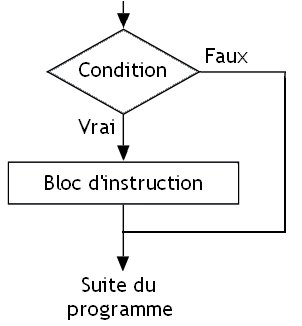
\includegraphics[scale=0.4]{images/boucle_condition.jpg}
\caption{Structure If}
\end{figure}

L'instruction \mybox{if} ressemble à ceci.

\begin{C}
if (/* Condition */)
{
    /* Une ou plusieurs instruction(s) */
}
\end{C}

Si la condition n'est pas vérifiée, le bloc d'instructions est passé et
le programme recommence immédiatement à la suite du bloc d'instructions
délimité par l'instruction \mybox{if}.

Si vous n'avez qu'une seule instruction à réaliser, vous avez la
possibilité de ne pas mettre d'accolades.

\begin{C}
if (/* Condition */)
    /* Une seule instruction */
\end{C}

Cependant, nous vous conseillons de mettre les accolades
systématiquement afin de vous éviter des problèmes si vous décidez de
rajouter des instructions par la suite en oubliant d'ajouter des
accolades. Bien sûr, ce n'est qu'un conseil, vous êtes libre de ne pas
le suivre.

À présent, voyons quelques exemples d'utilisation.

\subsubsection{Exemple 1}
\label{exemple-1}

\begin{C}
#include <stdio.h>


int main(void)
{
    int a = 10;
    int b = 20;

    if (a < b)
    {
        printf("%d est inférieur à %d\n", a, b);
    }

    return 0;
}
\end{C}

\begin{C}
10 est inférieur à 20
\end{C}

L'instruction \mybox{if} évalue l'expression logique
\mybox{a\ \textless{}\ b}, conclut qu'elle est valide et exécute le
bloc d'instructions.

\subsubsection{Exemple 2}
\label{exemple-2}

\begin{C}
#include <stdio.h>


int main(void)
{
    int a = 10;
    int b = 20;

    if (a > b)
    {
        printf("%d est supérieur à %d\n", a, b);
    }

    return 0;
}
\end{C}

Ce code n'affiche rien. La condition étant fausse, le bloc contenant
l'appel à la fonction \mybox{printf()} est ignoré.

\subsection{L'instruction else}
\label{linstruction-else}

Avec l'instruction \mybox{if}, nous savons exécuter un bloc
d'instructions quand une condition est remplie. Toutefois, si nous
souhaitons réaliser une action en cas d'échec de l'évaluation de la
condition, nous devons ajouter une autre instruction \mybox{if} à la
suite, comme ci-dessous.

\begin{C}
if (a > 5)
{
    /* Du code */
}

if (a <= 5)
{
    /* Code alternatif */
}
\end{C}

Le seul problème, c'est qu'il est nécessaire d'ajouter une instruction
\mybox{if} et d'évaluer une nouvelle condition, ce qui n'est pas très
efficace et assez long à taper. Pour limiter les dégâts, le C fournit
une autre instruction : \mybox{else}, qui signifie « sinon ». Celle-ci
se place immédiatement après le bloc d'une instruction \mybox{if} et
permet d'exécuter un bloc d'instructions alternatif si la condition
testée n'est pas vérifiée. Sa syntaxe est la suivante.

\begin{C}
if (/* Condition */)
{
    /* Une ou plusieurs instructions */
}
else
{
    /* Une ou plusieurs instructions */
}
\end{C}

Et elle doit être comprise comme ceci.

\begin{figure}[htbp]
\centering
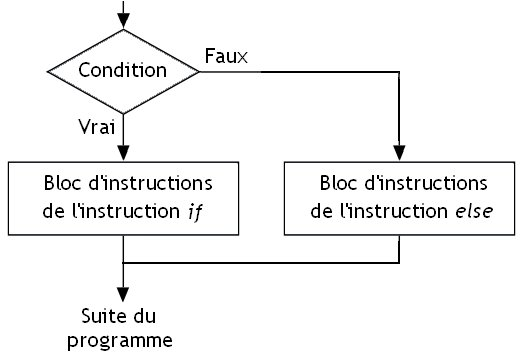
\includegraphics[scale=0.4]{images/boucle_if_else.jpg}
\caption{Structure if else}
\end{figure}

\begin{infobox} Notez que l'instruction \mybox{else}
ne possède aucune parenthèse.
\end{infobox}

\subsection{Exemple}
\label{exemple-3}

Supposons que nous voulions créer un programme très simple auquel nous
fournissons une heure et qui indique s'il fait jour ou nuit à cette
heure-là. Nous supposerons qu'il fait jour de 8 heures à 20 heures et
qu'il fait nuit sinon.

\begin{C}
int main(void)
{
    int heure;
    scanf("%d", &heure);

    if (heure > 8 && heure < 20)
    {
        printf("Il fait jour.\n");
    }
    else
    {
        printf("Il fait nuit.\n");
    }

    return 0;
}
\end{C}

\begin{C}
10
Il fait jour.
\end{C}

\section{If / else if}
\label{if-else-if}

Il est parfois nécessaire d'imbriquer plusieurs instructions \mybox{if}
et \mybox{else} les unes dans les autres.

\begin{C}
if (/* Condition */)
{
    /* Du code */
}
else
{
    /* Une ou plusieurs instruction(s) */

    if (/* Autre condition */)
    {
        /* Du code */
    }
}
\end{C}

Cependant, c'est assez long à écrire, d'autant plus s'il y a beaucoup
d'imbrications. Pour éviter ces inconvénients, sachez qu'il est possible
de combiner une instruction \mybox{else} et une instruction
\mybox{if}. Les imbrications simplifiables avec une suite \mybox{else}
\mybox{if} sont celles qui s'écrivent comme suit.

\begin{C}
if (/* Expression logique */)
{
    /* Une ou plusieurs instruction(s) */
}
else 
{
    if (/* Expression logique */)
    {
        /* Une ou plusieurs instruction(s) */
    }
}
\end{C}

Faites bien attention : le bloc d'instructions du \mybox{else} doit
contenir un \mybox{if}, éventuellement avec un \mybox{else}, mais rien
d'autre. Celles-ci peuvent alors être simplifiées comme ceci.

\begin{C}
if (/* Expression logique */)
{
    /* Une ou plusieurs instruction(s) */
}
else if (/* Expression logique */)
{
    /* Une ou plusieurs instruction(s) */
}
\end{C}

Comme vous pouvez le voir, nous avons « fusionné » l'instruction
\mybox{else} et la seconde instruction \mybox{if}. Notez que comme il
s'agit toujours d'une suite d'instructions \mybox{if} et \mybox{else},
il n'y aura qu'un seul bloc d'instructions qui sera finalement exécuté.
En effet, l'ordinateur va tester la condition de l'instruction
\mybox{if}, puis, si elle est fausse, celle de l'instruction
\mybox{if} suivant l'instuction \mybox{else} et ainsi de suite jusqu'à
ce qu'une condition soit vraie (ou jusqu'à une instruction \mybox{else}
finale si elles sont toutes fausses).

\begin{infobox} Notez qu'il n'est pas obligatoire
d'ajouter une instruction \mybox{else}.
\end{infobox}

\begin{C}
#include <stdio.h>


int main(void)
{
    int heure = 11;

    if (heure < 7)
    {
        printf("Zzz... \n");
    }
    else if (heure >= 7 && heure < 12)
    {
        printf("C'est le matin !\n");
    }
    else if (heure == 12)
    {
        printf("Il est midi !\n");
    }
    else if (heure > 12 && heure < 18)
    {
        printf("C'est l'après-midi !\n");
    }
    else if (heure >= 18 && heure < 24)
    {
        printf("C'est le soir !\n");
    }
    else if (heure == 24 || heure == 0)
    {
        printf("Il est minuit, dormez brave gens !\n");
    }
    else
    {
        printf("Il est l'heure de réapprendre à lire l'heure !\n");
    }

    return 0;

\end{C}

\begin{C}
11
On est le matin !
0
Il est minuit, dormez brave gens !
-2
Il est l'heure de réapprendre à lire l'heure !
\end{C}

\subsection{Exercice}
\label{exercice-1}

Imaginez que vous avez un score de jeu vidéo sous la main :

\begin{itemize}
\item
  si le score est strictement inférieur à deux mille, affichez « C'est
  la catastrophe ! » ;
\item
  si le score est supérieur ou égal à deux mille et que le score est
  strictement inférieur à cinq mille, affichez : « Tu peux mieux faire
  ! » ;
\item
  si le score est supérieur ou égal à cinq mille et que le score est
  strictement inférieur à neuf mille, affichez : « Tu es sur la bonne
  voie ! » ;
\item
  sinon, affichez : « Tu es le meilleur ! ».
\end{itemize}

Au boulot !

\begin{C}
 #include <stdio.h>


int main(void)
{
    int score;

    printf("Quel est le score du joueur ? ");
    scanf("%d", &score);

    if (score < 2000)
    {
        printf("C'est la catastrophe !\n");
    }
    else if (score >= 2000 && score < 5000)
    {
        printf("Tu peux mieux faire !\n");
    }
    else if (score >= 5000 && score < 9000)
    {
        printf("Tu es sur la bonne voie !\n");
    }
    else
    {
        printf("Tu es le meilleur !\n");
    }

    return 0;
}
\end{C}


\section{L'instruction switch}
\label{linstruction-switch}

L'instruction \mybox{switch} permet de comparer la valeur d'une
variable par rapport à une liste de valeurs. Techniquement, elle permet
d'écrire de manière plus concise une suite d'instructions \mybox{if} et
\mybox{else} qui auraient pour objectif d'accomplir différentes actions
suivant la valeur d'une variable.

\begin{C}
if (a == 1)
{
    /* Instruction(s) */
}
else if (a == 2)
{
    /* Instruction(s) */
}
/* Etc. */
else
{
    /* Instruction(s) */
}
\end{C}

Avec l'instruction \mybox{switch}, cela donne ceci.

\begin{C}
switch (a)
{
case 1:
    /* Instruction(s) */
    break;
case 2:
    /* Instruction(s) */
    break;

/* Etc... */

default: /* Si aucune comparaison n'est juste */
    /* Instruction(s) à exécuter dans ce cas */
    break;
}
\end{C}

Ici, la valeur de la variable \emph{a} est comparée successivement avec
chaque entrée de la liste, indiquées par le mot-clé \mybox{case}. En
cas de correspondance, les instructions suivant le mot-clé \mybox{case}
sont exécutées jusqu'à rencontrer une instruction \mybox{break} (nous
la verrons plus en détail un peu plus tard). Si aucune comparaison n'est
bonne, alors ce sont les instructions de l'entrée marquée avec le
mot-clé \mybox{default} qui seront exécutées.

\subsection{Exemple}
\label{exemple-4}

\begin{C}
#include <stdio.h>


int main(void)
{
    int note;

    printf("Quelle note as-tu obtenue (sur cinq) ? ");
    scanf("%d", &note);

    switch(note)
    {
    /* si note == 0 */
    case 0:
        printf("No comment.\n");
        break;

    /* si note == 1 */
    case 1:
        printf("Cela te fait 4/20, c'est accablant.\n");
        break;

    /* si note == 2 */   
    case 2:
        printf("On se rapproche de la moyenne, mais ce n'est pas encore ça.\n");
        break;

    /* si note == 3 */
    case 3:
        printf("Tu passes.\n");
        break;

    /* si note == 4*/
    case 4:
        printf("Bon travail, continue ainsi !\n");
        break;

    /* si note == 5 */
    case 5:
        printf("Excellent !\n");
        break;

    /* si note est différente de 0, 1, 2, 3, 4 et 5 */
    default:
        printf("Euh... tu possèdes une note improbable...\n");
        break;
    }

    return 0;
}
\end{C}

\begin{infobox} Notez que comme pour l'instruction
\mybox{else}, une entrée marquée avec le mot-clé \mybox{default} n'est
pas obligatoire.
\end{infobox}

\subsection{Plusieurs entrées pour une même action}
\label{plusieurs-entrees-pour-une-muxeame-action}

Une même suite d'instructions pour être désignée par plusieurs entrées
comme le montre l'exemple suivant.

\begin{C}
int main(void)
{
    int note;

    printf("Quelle note as-tu obtenue ? ");
    scanf("%d", &note);

    switch(note)
    {
    /* si la note est comprise entre zéro et trois inclus */
    case 0:
    case 1:
    case 2:
    case 3:
        printf("No comment.\n");
        break;

    /* si la note est comprise entre quatre et sept inclus */
    case 4:
    case 5:
    case 6:
    case 7:
        printf("C'est accablant.\n");
        break;

    /* si la note est comprise entre huit et neuf inclus */  
    case 8:
    case 9:
        printf("On se rapproche de la moyenne, mais ce n'est pas encore ça.\n");
        break;

    /* si la note est comprise entre dix et douze inclus */
    case 10:
    case 11:
    case 12:
        printf("Tu passes.\n");
        break;

    /* si la note est comprise entre treize et seize inclus */
    case 13:
    case 14:
    case 15:
    case 16:
        printf("Bon travail, continue ainsi !\n");
        break;

    /* si la note est comprise entre dix-sept et vingt inclus */
    case 17:
    case 18:
    case 19:
    case 20:
        printf("Excellent !\n");
        break;

    /* si la note est différente */
    default:
        printf("Euh... tu possèdes une note improbable...\n");
        break;
    }

    return 0;
}
\end{C}

\section{Plusieurs entrées sans instruction break}
\label{plusieurs-entrees-sans-instruction-break}

Si vous l'utiliserez souvent, sachez également que l'instruction
\mybox{break} n'est pas obligatoire. En effet, le but de cette dernière
est de sortir du \mybox{switch} et donc de ne pas exécuter les actions
d'autre entrées. Toutefois, il arrive que les actions à réaliser se
chevauchent entre entrées auquel cas l'instruction \mybox{break} serait
plutôt mal venue.

Prenons un exemple : vous souhaitez réaliser un programme qui affiche
entre 1 à dix fois la même phrase, ce nombre étant fourni par
l'utilisateur. Vous pourriez écrire une suite de \mybox{if} ou
différentes entrées d'un \mybox{switch} qui, suivant le nombre entré,
appelleraient une fois \mybox{printf()}, puis deux fois, puis trois
fois, etc. mais cela serait horriblement lourd.

Dans un tel cas, une meilleure solution consiste à appeler
\mybox{printf()} à chaque entrée du \mybox{switch}, mais de ne pas
terminer ces dernières par une instruction \mybox{break}.

\begin{C}
#include <stdio.h>


int
main(void)
{
    unsigned nb;

    printf("Combien de fois souhaitez-vous répéter l'affichage (entre 1 à 10 fois) ? ");
    scanf("%u", &nb);

    switch (nb)
    {
    case 10:
        printf("Cette phrase est répétée une à dix fois.\n");
    case 9:
        printf("Cette phrase est répétée une à dix fois.\n");
    case 8:
        printf("Cette phrase est répétée une à dix fois.\n");
    case 7:
        printf("Cette phrase est répétée une à dix fois.\n");
    case 6:
        printf("Cette phrase est répétée une à dix fois.\n");
    case 5:
        printf("Cette phrase est répétée une à dix fois.\n");
    case 4:
        printf("Cette phrase est répétée une à dix fois.\n");
    case 3:
        printf("Cette phrase est répétée une à dix fois.\n");
    case 2:
        printf("Cette phrase est répétée une à dix fois.\n");
    case 1:
        printf("Cette phrase est répétée une à dix fois.\n");
    case 0:
        break;
    default:
        printf("Certes, mais encore ?\n");
        break;
    }

    return 0;
}
\end{C}

\begin{C}
Combien de fois souhaitez-vous répéter l'affichage (entre 1 à 10 fois) ? 2
Cette phrase est répétée une à dix fois.
Cette phrase est répétée une à dix fois.

Combien de fois souhaitez-vous répéter l'affichage (entre 1 à 10 fois) ? 5
Cette phrase est répétée une à dix fois.
Cette phrase est répétée une à dix fois.
Cette phrase est répétée une à dix fois.
Cette phrase est répétée une à dix fois.
Cette phrase est répétée une à dix fois.
\end{C}

Comme vous le voyez, la phrase « Cette phrase est répétée une à dix fois
» est affichée une à dix fois suivant le nombre initialement fourni.
Cela est possible étant donné l'absence d'instruction \mybox{break}
entre les \mybox{case} 10 à 1, ce qui fait que l'exécution du
\mybox{switch} continue de l'entrée initiale jusqu'au \mybox{case} 0.

\section{L'opérateur conditionnel}
\label{loperateur-conditionnel}

L'\textbf{opérateur conditionnel} ou \textbf{opérateur ternaire} est un opérateur
particulier dont le résultat dépend de la réalisation d'une condition.
Son deuxième nom lui vient du fait qu'il est le seul opérateur du
langage C à requérir trois opérandes : une condition et deux
expressions.

\begin{C}
(condition) ? expression si vrai : expression si faux
\end{C}

\begin{infobox}
Les parenthèses entourant la
condition ne sont pas obligatoires, mais préférables.
\end{infobox}

\emph{Grosso modo}, cet opérateur permet d'écrire de manière condensée
une structure \mybox{if\ \{\}\ else\ \{\}}. Voyez par vous-mêmes.

\begin{C}
#include <stdio.h>

int main(void)
{
    int heure;

    scanf("%d", &heure);

    (heure > 8 && heure < 20) ? printf("Il fait jour.\n") : printf("Il fait nuit.\n");
    return 0;
}
\end{C}

Il est également possible de l'écrire sur plusieurs lignes, même si
cette pratique est moins courante.

\begin{C}
(heure > 8 && heure < 20)
    ? printf("Il fait jour.\n")
    : printf("Il fait nuit.\n");
\end{C}

Cet opérateur peut sembler inutile de prime abord, mais il s'avère être
un allié de choix pour simplifier votre code quand celui-ci requiert la
vérification de conditions simples.

\subsection{Exercice}
\label{exercice-2}

Pour bien comprendre cette nouvelle notion, nous allons faire un petit
exercice. Imaginez que nous voulions faire un mini jeu vidéo dans lequel
nous affichons le nombre de coups du joueur. Seulement voilà, vous êtes
maniaques du français et vous ne supportez pas qu'il y ait un « s » en
trop ou en moins. Essayez de réaliser un programme qui demande à
l'utilisateur d'entrer un nombre de coups puis qui affiche celui-ci
correctement accordé.

\begin{C}
 #include <stdio.h>

int main(void)
{
    int nb_coups;

    printf("Donnez le nombre de coups : ");
    scanf("%d", &nb_coups);
    printf("Vous gagnez en %d coup%c\n", nb_coups, (nb_coups > 1) ? 's' : ' ');
    return 0;
}
\end{C}

Ce programme utilise l'opérateur conditionnel pour condenser
l'expression et aller plus vite dans l'écriture du code. Sans lui nous
aurions dû écrire quelque chose comme ceci.

\begin{C}
 #include <stdio.h>

int main(void)
{
    int nb_coups;

    printf("Donnez le nombre de coups : ");
    scanf("%d", &nb_coups);

    if (nb_coups > 1)
        printf("Vous gagnez en %d coups\n", nb_coups);
    else
        printf("Vous gagnez en %d coup\n", nb_coups);

    return 0;
}
\end{C}

Ce chapitre a été important, il vous a permis d’utiliser les conditions ; les instructions \mybox{if} et \mybox{else};
l’instruction \mybox{switch} et l'opérateur conditionnel. Aussi, si vous n'avez pas très bien compris
ou que vous n'avez pas tout retenu, nous vous conseillons de relire ce
chapitre.

Le chapitre suivant sera l'occasion de mettre en œuvre ce que vous avez
appris puisqu'il s'agira de votre premier TP.

*{[}TP{]}: Travaux Pratiques